\documentclass{report}
\usepackage{graphicx}
\usepackage{amsmath}
\usepackage{algorithmic}
\usepackage{algorithm}
\usepackage{booktabs}
\usepackage{caption}
\usepackage{shadowtext}
\usepackage[margin=1in]{geometry}


\usepackage[colorlinks=true, linkcolor=blue, citecolor=blue, urlcolor=blue]{hyperref}

\begin{document}
	
	\begin{titlepage}
		\centering
		
\includegraphics[width=0.15\textwidth]{./assets/bw_kiit.png}\par\vspace{1cm}
		{\LARGE \textsc{Kalinga Institute of Industrial Technology}\par}
		{\textsc{Deemed to be University}\par}
		\vspace{1cm}
		{\Large \textsc{Lab Mini Project 4}\par}
		\vspace{1.5cm}
		{\huge\shadowtext{\textsc{AI Laboratory}}\par}
		\vspace{1cm}
		\begin{tabular}{ll}
			\textsc{Aman Pathak}       & 22051662 \\
		\end{tabular}
		\vspace{0.5cm}					
		\vfill
		supervised by\par
		Dr.~Sambit \textsc{Praharaj}
		
		\vfill
		
		% Bottom of the page
		{\large \today\par}
	\end{titlepage}
	
	
	
	\chapter{N-Queens Problem Solution Using Hill Climbing}
	
	\section{Introduction}
	The N-Queens problem serves as a classical constraint satisfaction problem where the objective is to place N queens on an N×N chessboard such that no two queens threaten each other. This chapter presents an implementation of the Hill Climbing algorithm to solve the N-Queens problem, complete with a graphical user interface for visualization and performance analysis.
	
	\section{System Architecture}
	The implementation consists of three core components: the solver module, visualizer module, and GUI interface. The solver module implements the Hill Climbing algorithm with fitness evaluation and neighbor generation. The visualizer module uses Pygame to render the chessboard and queen placements dynamically. The GUI, built with CustomTkinter, provides user control over parameters and displays performance metrics including execution time and memory consumption.
	
	\section{Algorithm Implementation}
	The Hill Climbing implementation begins with random initialization of queens, one per column. The fitness function calculates pairwise conflicts between queens, counting attacks along rows and diagonals. Neighbor generation moves one queen at a time within its column, creating all possible adjacent states. The algorithm iteratively selects the best neighbor until no improvement is found, reaching either a global optimum (zero conflicts) or local optimum (non-zero conflicts).
	
	The time complexity is O(N\textsuperscript{3}) per iteration due to the fitness calculation over N queens. Space complexity is O(N\textsuperscript{2}) for storing the board state. Memory usage scales quadratically with N due to the chessboard representation and path storage for visualization.
	
	\section{Performance Analysis}
	Table \ref{tab:performance} presents empirical measurements across different problem sizes. The solution consistently finds global optima for smaller boards ($N \le 8$) but encounters local optima for larger instances. Memory usage grows polynomially with N, while execution time shows exponential characteristics due to the expanding search space.
	
	\begin{table}[h]
		\centering
		\caption{Performance Metrics for Various Board Sizes}
		\label{tab:performance}
		\begin{tabular}{ccccc}
			\toprule
			\textbf{N} & \textbf{Time (s)} & \textbf{Memory (MB)} & \textbf{Fitness} & \textbf{Solution Found} \\
			\midrule
			8 & 0.01 & 0.13 & 0 & True \\
			16 & 0.17 & 1.52 & 2 & False \\
			32 & 7.04 & 20.58 & 5 & False \\
			\bottomrule
		\end{tabular}
	\end{table}
	
	\section{Visualization Interface}
	The GUI (Figure \ref{fig:gui}) provides interactive control over board size and animation speed. The visualizer (Figure \ref{fig:visualizer}) renders each intermediate state during the search process, showing queen placements on a chessboard with alternating green and white squares. The animation time step is configurable, allowing observation of the algorithm's progression.
	
	\begin{figure}[h]
		\centering
		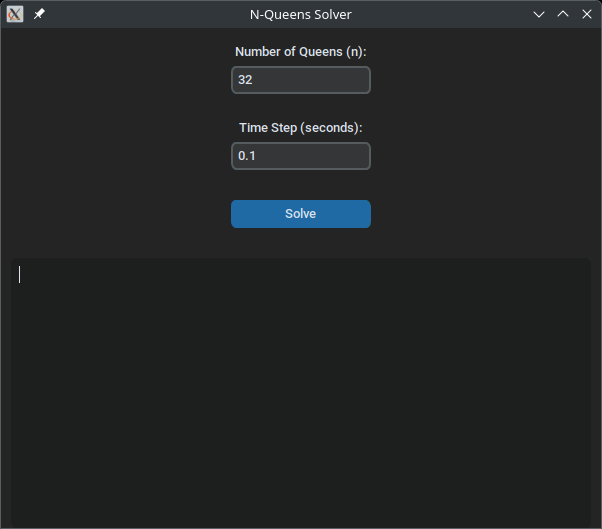
\includegraphics[width=0.4\textwidth]{assets/gui.png}
		\caption{GUI Interface for N-Queens Solver}
		\label{fig:gui}
	\end{figure}
	
	
	
	\begin{figure}[h]
		\centering
		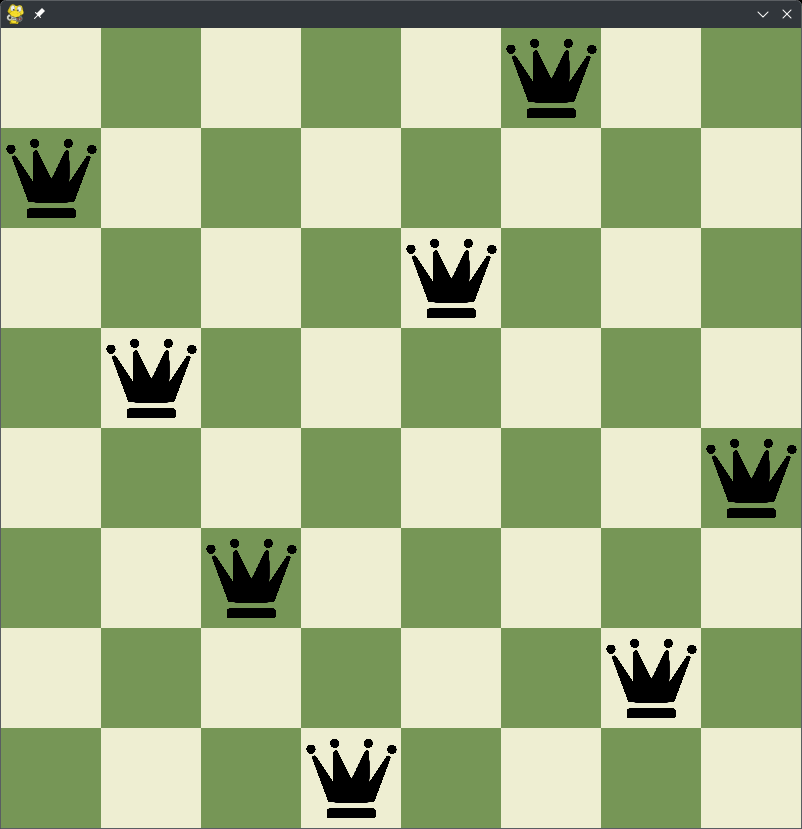
\includegraphics[width=0.6\textwidth]{assets/solver.png}
		\caption{Board State Visualization}
		\label{fig:visualizer}
	\end{figure}
	
	
	
	\section{Limitations and Improvements}
	The current implementation demonstrates the fundamental limitations of Hill Climbing: susceptibility to local optima and poor scalability. For N=32, the algorithm fails to find a solution within reasonable time while consuming significant memory. Potential improvements include incorporating random restarts, simulated annealing for probabilistic neighbor acceptance, or hybrid approaches combining local search with constraint propagation.
	
	The visualization component currently loads all states into memory before rendering, which becomes impractical for large N. A streaming implementation that generates states on-demand would improve memory efficiency for larger board sizes.
	
	
	
	
	
	\chapter{Hill Climbing for Feature Selection in Machine Learning}
	
	\section{Introduction}
	Feature selection constitutes a critical preprocessing step in machine learning pipelines, particularly for high-dimensional datasets where irrelevant or redundant features may degrade model performance. This chapter presents a Hill Climbing approach for feature subset selection, demonstrating its efficacy on the Ionosphere dataset from OpenML. The algorithm identifies an optimal feature subset that maximizes classification accuracy while reducing dimensionality, proving especially valuable in domains lacking prior feature importance knowledge.
	
	\section{Methodology}
	The implementation follows a structured six-step process: dataset loading, evaluation metric definition, initial subset generation, neighbor generation, Hill Climbing optimization, and performance comparison. The core algorithm operates on feature subsets represented as sets of indices, with the evaluation metric being classification accuracy from a Decision Tree classifier. Neighbor generation creates adjacent states by either adding or removing single features from the current subset.
	
	The fitness function $f(S)$ for a feature subset $S$ is defined as:
	\begin{equation}
		f(S) = \texttt{accuracy\_score}(\text{DecisionTreeClassifier}(X_S), y)
	\end{equation}
	where $X_S$ represents the dataset projected onto features in $S$. The algorithm terminates when no neighboring subset yields improved accuracy, reaching a local maximum in the feature subset space.
	
	\section{Technical Implementation}
	The Python implementation uses scikit-learn for model evaluation and NumPy for efficient subset operations. Key components include:
	
	The neighbor generation function explores the feature space by producing all possible subsets differing by exactly one feature from the current solution. This creates a search space of size $2^d$ where $d$ is the total number of features. The Hill Climbing implementation employs a greedy first-improvement strategy, moving to the first better neighbor found rather than exhaustively evaluating all neighbors.
	
	Memory efficiency is maintained by storing only feature indices rather than copying data matrices during the search. The evaluation function uses a 70-30 train-test split with fixed random state for reproducible accuracy measurements. Decision Trees serve as the evaluation model due to their sensitivity to irrelevant features and computational efficiency.
	
	\section{Results and Analysis}
	The algorithm identified an optimal feature subset comprising indices \{9, 11, 12, 18, 22, 23, 26, 29\} achieving 94.34\% accuracy, outperforming the full feature set accuracy of 89.62\%. This demonstrates the method's ability to eliminate noisy or redundant features while improving model performance. Table \ref{tab:feature_results} contrasts the performance metrics.
	
	\begin{table}[h]
		\centering
		\caption{Feature Selection Performance Comparison}
		\label{tab:feature_results}
		\begin{tabular}{lcc}
			\toprule
			\textbf{Configuration} & \textbf{Feature Count} & \textbf{Accuracy (\%)} \\
			\midrule
			All Features & 34 & 89.62 \\
			Optimal Subset & 8 & 94.34 \\
			\bottomrule
		\end{tabular}
	\end{table}
	
	\section{Dimensionality Reduction Benefits}
	The solution provides significant dimensionality reduction, decreasing the feature space from 34 to 8 dimensions (76.5\% reduction) while improving accuracy by 4.72 percentage points. This demonstrates Hill Climbing's effectiveness for feature selection when:
	
	The problem domain lacks established feature importance knowledge. The original feature space contains substantial redundancy or noise. Computational constraints necessitate smaller feature sets. Model interpretability benefits from reduced dimensionality. The method proves particularly valuable in exploratory data analysis phases where exhaustive feature evaluation is computationally prohibitive.
	
	\section{Limitations and Extensions}
	The current implementation exhibits several limitations characteristic of basic Hill Climbing: susceptibility to local optima and dependence on initial random subsets. Potential enhancements include:
	
	Incorporating simulated annealing to escape local optima. Implementing beam search to maintain multiple candidate solutions. Adding wrapper methods for more robust accuracy estimation. Including regularization terms in the fitness function to prevent overfitting. Parallel evaluation of neighbors could improve computational efficiency for larger feature spaces.
	
	The algorithm's linear neighbor generation strategy may become inefficient for extremely high-dimensional datasets ($d > 1000$). Future work could explore stochastic neighbor generation or feature space partitioning techniques to address this scalability challenge.
	
	
	
\end{document}